% Scalar instruction entry source: tools/generate_scalar_instruction_catalog.py.
\subsection{\texttt{LHI.U}}
\label{sec:scalar-lhi_u}
\index{LHI.U@\texttt{LHI.U}}
\begin{sloppypar}\noindent\textbf{Purpose.} Loads a signed 16-bit value from memory using unscaled immediate-offset addressing and writes the result to the selected destination.\end{sloppypar}\smallskip
\noindent\textbf{Syntax.}\par
\begin{lstlisting}[style=ptoscalarcode]
lhi.u [SrcL, simm], ->RegDst
\end{lstlisting}
\noindent\textbf{Encoding.}\par
\noindent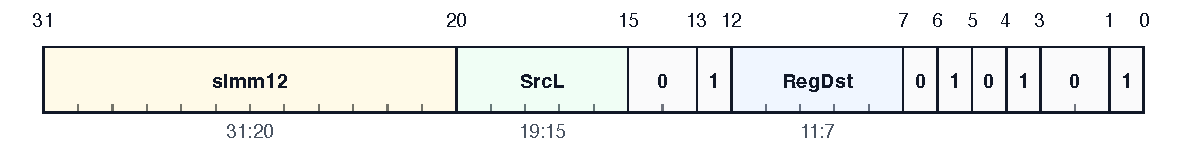
\includegraphics[width=\textwidth]{figs/encoding/scalar_instruction_entries/enc_lhi_u.pdf}\par\smallskip
\begin{description}[leftmargin=0.18\linewidth,style=nextline]
\item[Format] \texttt{L32} \texttt{32-bit} scalar word.
\item[Pattern] \texttt{.................001.....0101001}.
\end{description}
\noindent\textbf{Classification.}\par
\begin{description}[leftmargin=0.18\linewidth,style=nextline]
\item[Category] Load, Store, and Address Generation.
\item[Family] Load UnScaled.
\item[Execution class] \texttt{LDA/UNSCALED}; uop\_kind=AGU, agu\_kind=LDA, addr\_mode=UNSCALED.
\end{description}
\noindent\textbf{Operand fields.}\par
\begin{description}[leftmargin=0.18\linewidth,style=nextline]
\item[\texttt{RegDst}] Bits \texttt{11:7 (5b)}. 5-bit scalar destination register that receives the loaded value after any sign or zero extension; X0 discards the load result.
\item[\texttt{SrcL}] Bits \texttt{19:15 (5b)}. 5-bit scalar source register used as the base address for the memory access.
\item[\texttt{simm12}] Bits \texttt{31:20 (12b)}. 12-bit signed address displacement added to the base register to form the effective address.
\end{description}
\noindent\textbf{Operation.}\par
\begin{lstlisting}[style=ptoscalarcode]
addr = ComputeAddress(/* per syntax */)
value = Load16(addr)
value = SignExtend(value)
Write(RegDst, value)
\end{lstlisting}
\Needspace{0.08\textheight}
